\documentclass[thesis.tex]{subfiles}

\section{Problem Statement}
\subsection{Large-scale Training of Neural Networks}
Deep neural networks (DNNs) have seen drastic progress within the past several years. Improvements in network architecture and hardware capabilities have resulted in state-of-the-art performance in many cognitive tasks, most notably in computer vision, natural language processing and audio processing.

Training neural networks is a very computationally intensive tasks, which can take days or even weeks to complete. This makes experimenting and optimizing them very difficult. However, as DNNs process training examples in batches, they can be very scalable. Therefore, a framework that provides the capacity for large scale training can greatly improve training speed, and consequently network quality.

At the same time, distributed environments make it difficult to validate and test new networks. A preferable workflow would be testing a network locally, and deploying to multiple nodes later. As such, minimizing the amount of work required to port between these workflows is also a priority. This thesis aims to design and implement a system that satisfies these criterias.

\subsection{Object Detection}
Object detection is a computer vision problem that aims to detect instances of semantic objects of a certain class (such as humans, buildings, cars, etc...) in digital images and videos. Formally, object detection is often defined as: given an input image, produce a correct set of bounding boxes and corresponding labels for each defined object within the image. An example is shown in Figure \ref{fig:obj_example}.

\begin{figure}[htp]
	\centering
	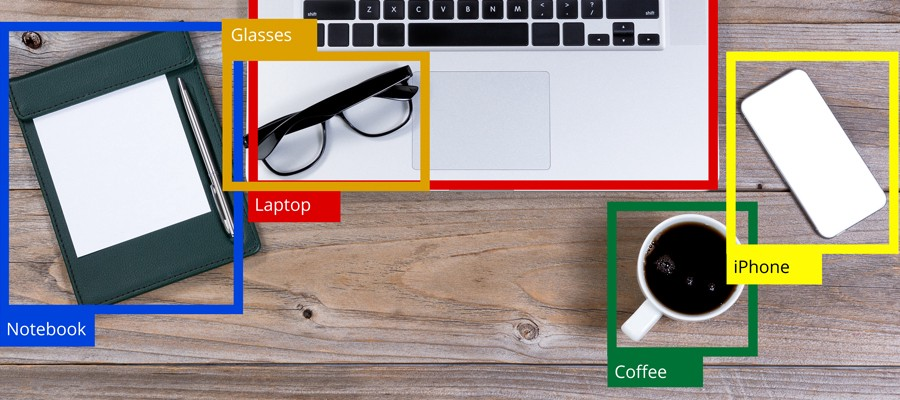
\includegraphics[width=0.7\textwidth]{obj_detection_example.jpeg}
	\caption{An example of object detection}
	\label{fig:obj_example}
\end{figure}

Object detection has a wide range of applications, most notably in surveillance (detecting people, movement,...) and image retrieval (using detected objects as image tags). It is also commonly applied in conjunction with other computer vision tasks, such as classification, eg. an object of a generic class may be detected and then further classified.

The more difficult task of finding the exact bound for objects (as opposed to bounding boxes) is called semantic segmentation.

\subsubsection{Detecting Document Text Regions}
Physical documents, such as books, reports, receipts,... still hold a large amount of information that's often inaccessible to computers. Digitizing these documents can open up a lot of possible applications, such as archiving historic texts, automatically grading exams, or managing personal finance.

An important task in digitizing these documents is finding the text regions. For documents with diverse structures (such as receipts or flyers), this is not trivial.

This thesis approaches the text region detection problem as an object detection problem. We use this problem as a case study to showcase the use of our framework.
